A continuación, se definen algunos conceptos que intervienen con el desarrollo del presente proyecto.

\section{Comunicación}

Los científicos han estudiado el porqué de las relaciones complejas entre los humanos en comparación a la complejidad presentada en las relaciones entre otros animales. Una de las hipótesis, Social Brain Hypothesis (SBH) postula que el crecimiento cognitivo humano y sus intrincadas relaciones sociales se deben a “la necesidad de nuestros ancestros de mantener e incrementar el número de relaciones sociales con diferentes grupos para sobrevivir en las extremadamente desafiantes condiciones ambientales originadas durante la última era glacial”.\cite{dynamics}

El hombre, en su continua evolución, ha utilizado el lenguaje como una herramienta creadora de conocimiento transferible a sus congéneres o cualquier otro ser que interactuase con él. Con esto, “los humanos han desarrollado el lenguaje como un instrumento ligero y conveniente para mantener sus relaciones” \cite{dynamics}. 

En la comunicación entre congéneres, el lenguaje puede ser dividido en dos funciones: función de transmisión de información (gossip) y función de entendimiento del estado interno (estado mental) del congénere (mentalisation) \cite{dynamics}. Estas funciones de transmisión y entendimiento del otro han permitido que dos o varios humanos puedan asociarse entre sí formando redes sociales.


\subsection{Evolución de la web}

La evolución de los servicios proporcionados a través de internet ha sido drástica puesto que ha cambiado el modo de vida de las personas. En la figura \ref{fig:utilizacion_internet} se evidencia que el crecimiento de internet (de los servicios que en ella se soportan) se da en función de los servicios de conectividad social que son creados y soportados en ella. La web 1.0 fue utilizada en mayor medida por científicos para el intercambio de información en formato hipertexto. No había una interacción fuerte entre cada científico sino que ellos acudían a internet para buscar o poner a disposición material científico. Con la venida de la web 2.0 y la introducción de la interacción del usuario con la web, generando contenido en tiempo real, fueron creados servicios de redes sociales en-línea (OSN en inglés: On-line Social Network), produciendo una partición en los tipos de redes sociales. Así, las redes sociales a las que pertenece el ser humano en la era digital se dividieron convenientemente en “redes sociales fuera de línea” y “redes sociales en línea” (Offline Social Network y Online Social Network) \cite{dynamics}.

\begin{figure}[!htb]
  \begin{center}
    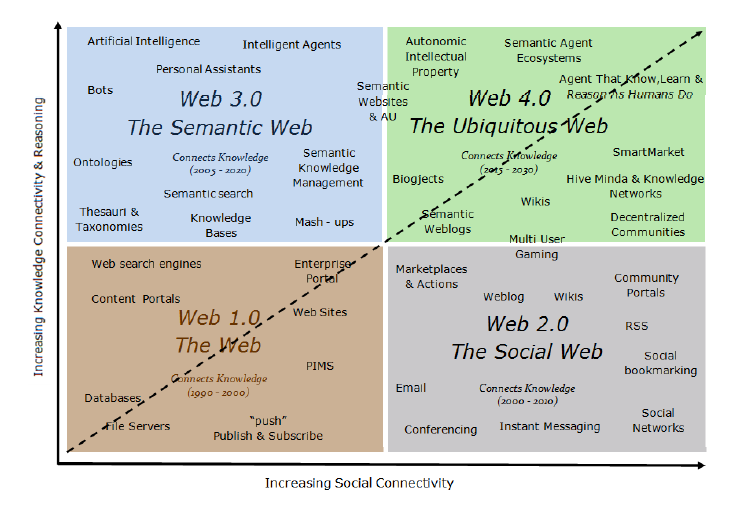
\includegraphics[width=11cm]{./imagenes/utilizacion_internet.png}
    \caption{Cambio de la utilización de internet en función de los servicios de conectividad social que son creados y soportados en ella}
    \label{fig:utilizacion_internet}
    \textbf{Fuente:}  http://goo.gl/3jGPPJ - Evolución de la web. Lozada, Pablo.
  \end{center}
\end{figure}


\section{Réd social}

La información contenida en la actual sección es tomada del libro \textit{Social Network Analisis for Startups} \cite{sna_startups}

Una red es un conjunto de relaciones. Mas específicamente, una red consiste en un conjunto de objetos (nodos) que están interconectados a través de relaciones (aristas). La red mas simple consiste en 2 nodos, N1 y N2, que están relacionados entre sí (Figura \ref{fig:simple}). Los nodos podrían representar personas, mientras la arista representa la relación que existe entre ellas (N1 y N2 son amigos, por ejemplo).

\begin{figure}[!htb]
  \begin{center}
    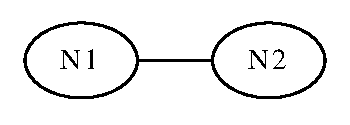
\includegraphics{./imagenes/Red_simple.eps}
    \caption{La red mas simple.}
    \label{fig:simple}
    \textbf{Fuente:}  Autores
  \end{center}
\end{figure}

Las redes sociales fuera de línea son las redes sociales que se forman por comunicación tradicional (lenguaje oral y escrito en medios que difieran de aquellos que utilizan las telecomunicaciones). Las redes sociales en línea son aquellas redes sociales que están formadas por cibernautas y en las cuales la comunicación se da por medio de los servicios de redes sociales. \cite{analysis}

Las relaciones pueden ser simétricas o asimétricas. Cuando se tiene una relación simétrica se dice que la relación no tiene dirección, es decir, la relación puede leerse en ambos sentidos. En el ejemplo anterior, significaría que N1 es amigo de N2 y que N2 es amigo de N1. Para que una relación se considere asimétrica, la relación debe poder leerse en un único sentido, es decir, la relación tiene una dirección determinada. En la figura \ref{fig:asimetrica} se puede observar un ejemplo de una red asimétrica en donde el nodo (o persona) N1 sigue al nodo N2, pero el nodo N2 no sigue al nodo N1.

\begin{figure}[!htb]
  \begin{center}
    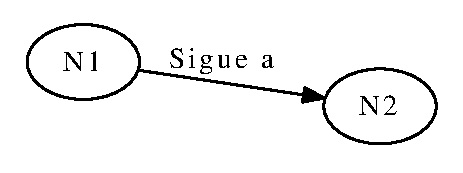
\includegraphics{./imagenes/Red_asimetrica.eps}
    \caption{Ejemplo de una red asimétrica.}
    \label{fig:asimetrica}
    \textbf{Fuente:}  Autores
  \end{center}
\end{figure}

Es posible que exista mas de una relación entre 2 nodos, en ese caso se dice que existe una \textit{relación multiplex} \cite[Cap.2]{cap_sna}


%\section{Business Process Modeling Notation (BPMN)}

%La información contenida en la actual sección es tomada del libro \textit{BPMN 2.0 Introduction to the Standard for Business Process Modeling} \cite{bpmn2}

%Al interior de una organización es importante documentar y especificar los diferentes procesos que se deben llevar a cabo. A menudo, se suelen utilizar diagramas de flujo o incluso descripciones textuales. Desafortunadamente, estas técnicas se quedan cortas a la hora de describir procesos mas complejos, y mas aún cuando cada organización define su propia notación, dificultando el entendimiento de los diferentes modelos que se realizan al interior de la organización. Es por esto que se hace necesario crear una notación estándar y especifica para describir este tipo de procesos.

%BPMN, Business Process Modeling Notation, es precisamente el estándar que se viene adoptando a nivel masivo para la creación y descripción de los diferentes procesos que hacen parte del funcionamiento de las diferentes organizaciones.


%Con el estándar BPMN, se tienen en cuenta diferentes elementos básicos que sirven como herramientas para crear y estructurar los diferentes modelos que se quieran hacer. Estos elementos solo describen una forma básica de uso, pues BPMN permite personalizar los elementos a utilizar, siempre y cuando los cambios realizados no dificulten el proceso de entendimiento de los modelos.

%\subsection{Pertinencia con el proyecto}

%Se utilizará BPMN como ayuda para el modelamiento de los diferentes procesos de negocio que sean identificados en la fase de análisis. Esto facilitará el proceso de diseño e implementación de los diferentes componentes necesarios para dar solución a los diferentes requerimientos del negocio.

\section{Service-Oriented Architecture (SOA)}

La información contenida en la actual sección es tomada del libro \textit{Soa principles of service design} \cite{soa_principles}

\subsection{Primeros conceptos}

Los conceptos base del diseño de software deben ser expuestos para tener una mayor claridad en los temas siguientes. A continuación se expresan los conceptos base:

\begin{itemize}
  \item \textbf{Características de diseño}: Son aquellos atributos que cumple un diseño y que pueden ser medidos.
  \item \textbf{Principio de diseño}: Es una guía o regla para solucionar un problema de acuerdo a las prácticas aceptadas por la comunidad de ingeniería de software.
  \item \textbf{Paradigma de diseño}: Es el compendio de principios de diseño que tienen un enfoque global común.
  \item \textbf{Patrones de diseño}: Son formas de resolver un problema de diseño que es repetitivo. Viene dado por 3 restricciones presentadas en el diseño de software:
  \begin{itemize}
    \item Restricciones impuestas por la tecnología existente
    \item Restricciones impuestas por las tecnologías usadas por sistemas transversales
    \item Restricciones de prioridades de proyectos
  \end{itemize}
  El patrón de diseño describe el problema y da la solución a modo de plantilla.
  \item \textbf{Lenguajes de patrones de diseño}: Es la configuración ordenada de patrones en un diseño lógico. La comunicación entre cada patrón se hace a través de dicho lenguaje.
  \item \textbf{Estándares de diseño}: En orden de ir acorde a las metas, prioridades, recursos y ambiente de la organización en la que se haga el diseño lógico de la solución, un estándar de diseño define convenciones para cada elemento utilizado en el diseño de acuerdo a las características de diseño definidas.
  \item \textbf{Buenas prácticas}: Es una técnica o acercamiento para resolver o prevenir problemas presentados en el desarrollo del diseño lógico de la solución de software. pg 34
\end{itemize}

\begin{figure}[!htb]
  \begin{center}
    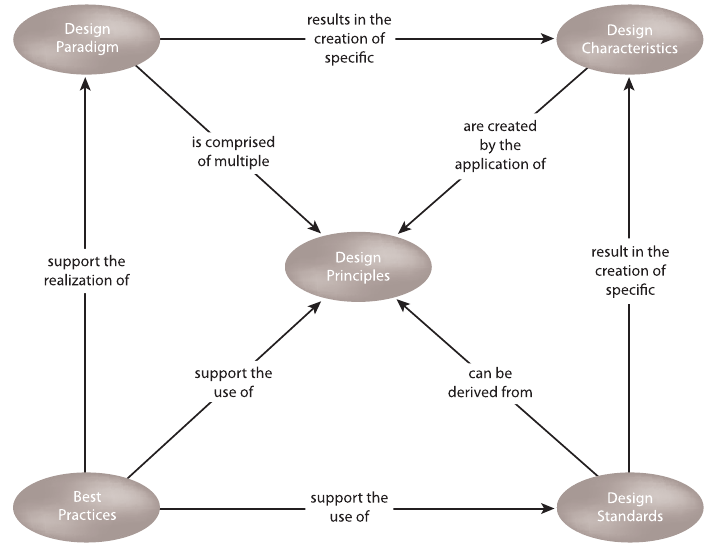
\includegraphics[width=11cm]{./imagenes/1.png}
    \caption{Acercamiento a cómo se desarrollan los principios de diseño con los demás conceptos nombrados.}
    \label{fig:uno}
    \textbf{Fuente:}  \cite{soa_principles}
  \end{center}
\end{figure}

La figura \ref{fig:uno} presenta un acercamiento a cómo se desarrollan los principios de diseño con los demás conceptos nombrados.

\begin{figure}[!htb]
  \begin{center}
    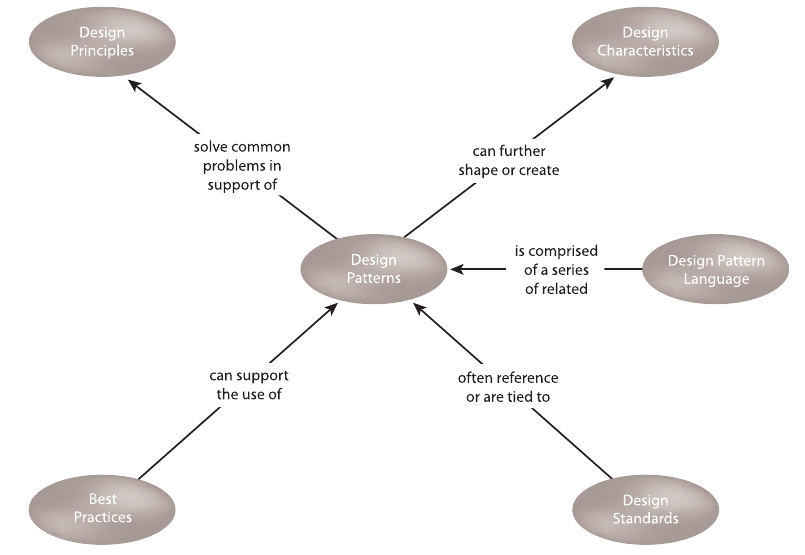
\includegraphics[width=11cm]{./imagenes/2.png}
    \caption{Como extiende o soporta un patrón de diseño el diseño lógico de la solución de software.}
    \label{fig:dos}
    \textbf{Fuente:}  \cite{soa_principles}
  \end{center}
\end{figure}

La figura \ref{fig:dos} presenta cómo extiende o soporta un patrón de diseño el diseño lógico de la solución de software.

\begin{figure}[!htb]
  \begin{center}
    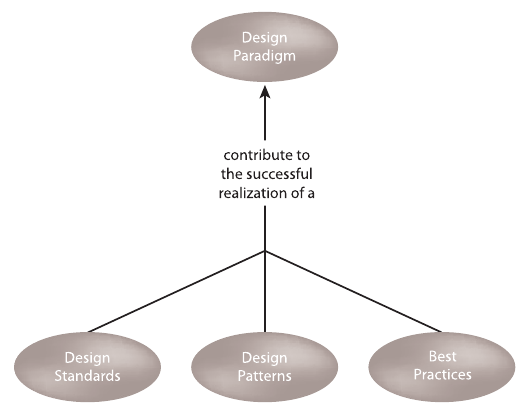
\includegraphics[width=11cm]{./imagenes/3.png}
    \caption{Componentes que hacen que el diseño lógico de la solución sea acorde al paradigma escogido.}
    \label{fig:tres}
    \textbf{Fuente:}  \cite{soa_principles}
  \end{center}
\end{figure}

La figura \ref{fig:tres} presenta los componentes que hacen que el diseño lógico de la solución sea acorde al paradigma escogido.

\subsection{Computación orientada a servicios}

La computación orientada a servicios nace de la necesidad de desarrollar software integrado con otros construidos con diferentes arquitecturas y, por ende, diversas tecnologías. Este tipo de computación tiene como finalidad la construcción de inventarios de servicios. La computación orientada a servicios está compuesta por la interacción de la orientación a servicios (paradigma de diseño) y la arquitectura orientada a servicios, formando patrones de diseño propios y estándares en cumplimiento de las características de diseño propias de la computación orientada a servicios. 

Algunos de los conceptos clave llevados en la computación orientada a servicios son:

\begin{itemize}
  \item Arquitectura Orientada a Servicios (SOA - Service Oriented Architecture): Comprende el compendio de tecnologías, APIs, infraestructura y repositorios enmarcados en el paradigma orientado a servicios y cuyo objetivo principal es el de trabajar sobre el "servicio" como el elemento más importante.
  \item Orientación a servicios: Es el paradigma manejado en la computación orientada a servicios en donde se acepta como unidad mínima y más importante el "servicio".
  \item Servicio: Es un software independiente físicamente el cual tiene asignado un contexto de funcionalidades y que puede ser utilizado por otros servicios por medio del contrato del servicio (descripción del servicio en cuanto a funcionalidades, entradas requeridas y salidas). De acuerdo a su nivel de reúso, los servicios se dividen en 3 tipos y son:
  \begin{itemize}
    \item Servicios entidad: Modela los servicios que se deben ofrecer respecto de las entidades del negocio (ej. empleados y clientes). Tienen un nivel de reúso alto y están centrados en el negocio.
    \item Servicios tarea: Modela los servicios que deben cumplir tareas específicas del negocio (ej. generación de cortes de final de año). Tienen un nivel de reúso bajo. Estos servicios trabajan directamente con 1 o varios servicios entidad. Estos servicios están centrados en el negocio.
    \item Servicios utilidad: Modela servicios que no están centrados en el negocio. Son los servicios con mayor reúso.
  \end{itemize}
\end{itemize}

\begin{figure}[!htb]
  \begin{center}
    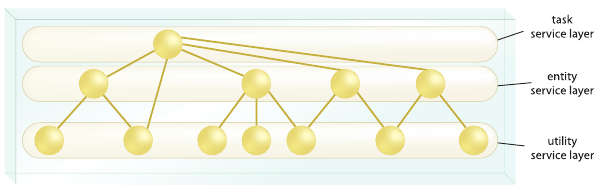
\includegraphics[width=11cm]{./imagenes/5.png}
    \caption{diferenciación entre tipos de servicio da lugar a la estructura en capas}
    \label{fig:cinco}
    \textbf{Fuente:}  \cite{soa_principles}
  \end{center}
\end{figure}

La diferenciación entre tipos de servicio da lugar a la estructura en capas mostrada en la figura \ref{fig:cinco}

\begin{itemize}
  \item Composición de servicios: Es la agregación de servicios de manera ordenada.
  \item Inventario de servicios: Es la agrupación de varios servicios según un criterio definido por la organización. Cada inventario de servicios tiene su propio estándar de diseño e, inclusive, su propia configuración arquitectónica. El desarrollo de los inventarios de servicio es hecho a modo top-down, con la construcción de blueprints, también llamados modelo de servicios de negocio o modelos de inventario de servicios.
\end{itemize}

\begin{figure}[!htb]
  \begin{center}
    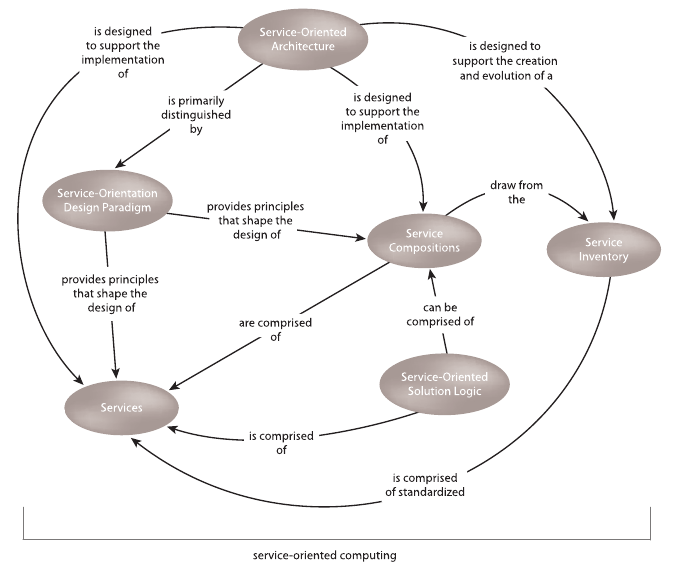
\includegraphics[width=11cm]{./imagenes/4.png}
    \caption{Interacción de los conceptos clave en la computación orientada a servicios}
    \label{fig:cuatro}
    \textbf{Fuente:}  \cite{soa_principles}
  \end{center}
\end{figure}

\subsection{Pertinencia con el proyecto}


La arquitectura base para la ejecución del proyecto es SOA. Esto brinda diferentes beneficios a la hora del desarrollo del proyecto, como los son:
\begin{itemize}
  \item Gracias al bajo acoplamiento conseguido con la arquitectura SOA, los componentes implementados son altamente reutilizables, lo que facilita y agiliza el proceso de desarrollo. Ademas,
  \item Es posible consumir servicios creados por terceros, limitando los servicios que deben ser creados a los que sean estrictamente de negocio.
\end{itemize}

\section{Scrum}

Sus creadores lo describen como “Un marco de trabajo por el cual las personas pueden acometer problemas complejos 
adaptativos, a la vez que entregar productos del máximo valor posible productiva y creativamente” \cite{scrum_guide}. Scrum se caracteriza por ser ágil, ligero, fácil de entender y difícil de llegar a dominar.

Scrum se basa en el empirismo, que dice que el conocimiento proviene de la experiencia, por lo que ``utiliza un enfoque iterativo e incremental para optimizar la predictibilidad y el control del riesgo'' \cite{scrum_guide}.

Los tres grandes pilares de la teoría de scrum son:

\begin{itemize}
  \item Transparencia: Todos los aspectos significativos deben ser visibles para sus stakeholders respectivos.

  \item Inspección: Los artefactos de scrum (y su progreso) deben ser inspeccionados frecuentemente para detectar variaciones. Estas inspecciones deben ser realizadas por un experto.

  \item Adaptación: Cuando una inspección detecta una variación que no cae en los limites permitidos, se deben hacer los reajustes necesarios para que el producto vuelva a rumbo deseado. Estos cambios deben hacerse lo más pronto posible, por esto las inspecciones deben ser realizadas de manera periódica a lo largo del desarrollo del proyecto.
\end{itemize}
